\documentclass[11pt, notitlepage,abstracton,oneside]{article}   	% use "amsart" instead of "article" for AMSLaTeX format
\usepackage{geometry}                		% See geometry.pdf to learn the layout options. There are lots.
\geometry{letterpaper}                   		% ... or a4paper or a5paper or ... 
\usepackage{graphicx}				% Use pdf, png, jpg, or eps§ with pdflatex; use eps in DVI mode
								% TeX will automatically convert eps --> pdf in pdflatex		
\usepackage{amssymb}

\title{Analysis of Medical Device Failure Reports from the MAUDE Database: A Data Mining Approach}
\author{Simon Diemert, Scott Low, Paul Moon}
\date{March 23rd 2015}							% Activate to display a given date or no date

\begin{document}
\maketitle

\begin{abstract}

%REFERENCE FORMAT: http://cs.stanford.edu/people/widom/paper-writing.html#related

\thispagestyle{empty}
Lorem Ipsum is simply dummy text of the printing and typesetting industry. Lorem Ipsum has been the industry's standard dummy text ever since the 1500s, when an unknown printer took a galley of type and scrambled it to make a type specimen book. It has survived not only five centuries, but also the leap into electronic typesetting, remaining essentially unchanged. It was popularised in the 1960s with the release of Letraset sheets containing Lorem Ipsum passages, and more recently with desktop publishing software like Aldus PageMaker including versions of Lorem Ipsum.
\end{abstract}

\tableofcontents

\clearpage
\newpage
\setcounter{page}{1}
\section{Introduction}
Modern medicine relies heavily on technology to support the delivery of treatments and care. These technologies are described by the umbrella term ``medical devices" which encompasses mechanical, electrical, software, or combination thereof devices that are used in medical care. The implications of these devices failing can range from minor annoyances to death. Adverse events related to medical devices in the United States are reported to the Food and Drug Administration (FDA), these reports are stored in the \textbf{Ma}nufacturer and \textbf{U}ser \textbf{F}acility \textbf{D}evice \textbf{E}xperience (MAUDE) database and are publicly accessibly. The MAUDE database contains approximately 3.7 million records dating back to 1991. 

Previous works have focused on analyzing the data in the MAUDE database to extract trends related to specific devices \cite{weber_preliminary_2011}. However, many of these analyses have been conducted using a manual review process that does not lend itself well to analyzing the large number of records available in the MAUDE database. The FDA has recently made the data accessible via its openFDA API which allows programmatic access to the data. To our knowledge, no work has been published using this new API to acquire a larger set of the data. 

Health care is a complex domain that requires medical devices to interact with humans in increasingly complicated ways. There are many examples of adverse medical events that were caused by a combination of a device and human users, Horsky conducted an analysis of such an event \cite{horsky_2005}. Safety analysis of medical devices must consider more than the device, it must also consider how the device interacts with human actors \cite{karsh_health_2010}. Leveson has presented general a model for analyzing the behaviour of complex sociotechnical systems called the STAMP model. The STAMP model describes a system as a feedback control loop with a controlled process being actuated and sensed by a human actor \cite{leveson_engineering_2012}. Work by Mason-Blakely and Weber has tailored this model for analysis of software in health care, is visible in Figure \ref{fig:stamp-emr} \cite{stamp_emr_2011}

\begin{figure}[ht]
	\centering
	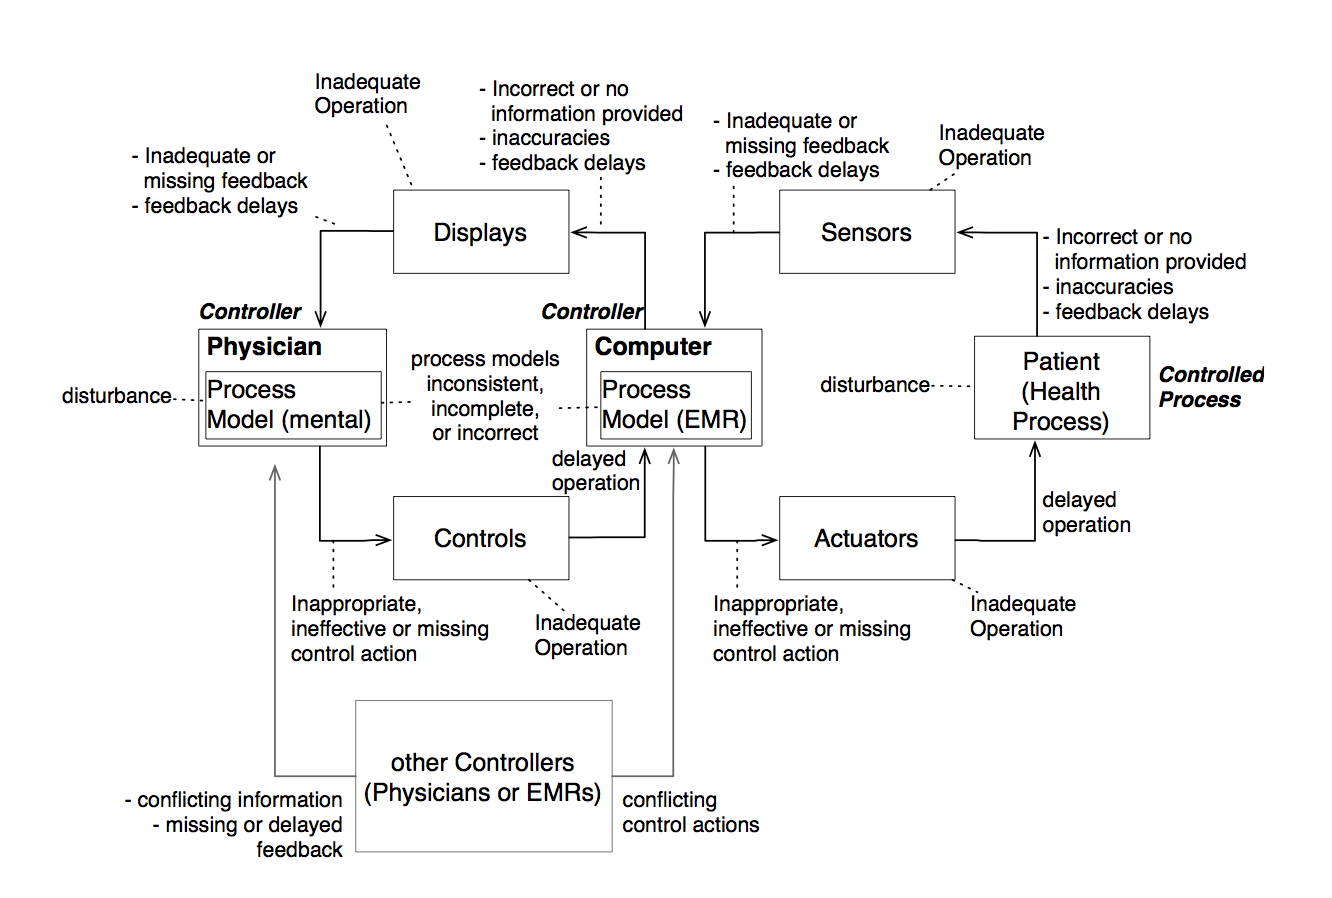
\includegraphics[width=0.95\textwidth]{figures/stamp-emr}
	\caption{STAMP - EMR model from \cite{stamp_emr_2011}}
	]\label{fig:stamp-emr}
\end{figure}

Mason-Blakey and Habibi used the STAMP EMR model to classify 350 adverse event reports related to software in the MAUDE database (not yet published). This classification was conducted by manually inspecting the natural language summary of each event. A number of different classes (related to the STAMP EMR model) were assigned to each record depending on the reviewer's understanding on the adverse event and how it fits into the STAMP EHR model. The categories used were: 

\begin{itemize}
	\item Care Provider
	\item Point of Care Sensor
	\item Point of Decision Display
	\item Point of Care Actuator
	\item Point of Decision Control
	\item Medical Device Decision Support (MDDS)
	\item Technical Process
\end{itemize}

In this project the MAUDE database was examined algorithmically using standard standard data mining techniques. Two different approaches were used to analyze data from MAUDE database:  i) analysis of the meta-data for each record to predict the outcome of the event (injury, death, etc.); ii) analyzed the natural language description of the adverse event to attempt to predict the categories (as outlined in the STAMP EMR model). The remainder of this paper is structured as follows: section 2 describes the methods used to collect and analyze this data; section 3 presents results; section 4 provides a discussion of results and outlines strengths and weaknesses of this approach. 

\section{Methods}

\subsection{Approach I: Meta Data Analysis}

\subsubsection{Data Collection}

\subsubsection{Data Pre-Processing}

\subsubsection{Data Analysis}

\subsection{Approach II: Record Categorization}
\subsubsection{Data Collection}

\subsubsection{Data Pre-Processing}

\subsubsection{Data Analysis}

\section{Results}

\subsection{Approach I: Meta Data Analysis}

\subsection{Approach II: Record Categorization}

\section{Discussion}
Lorem Ipsum is simply dummy text of the printing and typesetting industry. Lorem Ipsum has been the industry's standard dummy text ever since the 1500s, when an unknown printer took a galley of type and scrambled it to make a type specimen book. It has survived not only five centuries, but also the leap into electronic typesetting, remaining essentially unchanged. It was popularised in the 1960s with the release of Letraset sheets containing Lorem Ipsum passages, and more recently with desktop publishing software like Aldus PageMaker including versions of Lorem Ipsum.

\section{Conclusion}
Lorem Ipsum is simply dummy text of the printing and typesetting industry. Lorem Ipsum has been the industry's standard dummy text ever since the 1500s, when an unknown printer took a galley of type and scrambled it to make a type specimen book. It has survived not only five centuries, but also the leap into electronic typesetting, remaining essentially unchanged. It was popularised in the 1960s with the release of Letraset sheets containing Lorem Ipsum passages, and more recently with desktop publishing software like Aldus PageMaker including versions of Lorem Ipsum.


\bibliographystyle{plain}
\bibliography{report}


\end{document}  
